\chapter{Software for Practical, Reproducible Analysis}

\begin{center}
  \textit{When we had no computers, we had no programming problem either. 
    When we had a few computers, we had a mild programming problem. Confronted 
    with machines a million times as powerful, we are faced with a gigantic 
    programming problem.}

 - Edsger Dijkstra
\end{center}

Software plays an indispensable role in NMR data analysis, allowing us
to effectively manage and process massive data sets.  This chapter will
present several software projects that facilitate reproducible analysis.


\section{NMR-STAR library}
NMR-STAR is a file format used by the BMRB \cite{bmrb} for archival of
NMR data.  As such data is useful for further studies, and archiving
data in the BMRB is the primary means of dissemination, it is important
to be able to work with NMR-STAR files.

This library provides a robust interface for working with NMR-STAR files; 
it allows the creation of NMR-STAR files as well as extraction of data from 
existing files.

To handle these files, a library was implemented both in Java 
\cite{fenwick2013} and in Python.  This library provides capabilities both
for reading and for writing NMR-STAR files.  Although several tools for
dealing with NMR-STAR files had already been implemented \cite{ccpn, bmrb},
there are several attributes of this library which set it apart:
\begin{itemize}
  \item error reporting of illegal input.  When malformed input is encountered,
    a useful, location-specific error is reported which includes sufficient
    information to quickly pinpoint and diagnose the problem.
  \item complete, standards-compliant NMR-STAR syntax definition.
  \item open source under the MIT license.  This allows other interested 
    developers to inspect the source code to gain ideas, use the library in
    new applications, and modify and extend the library to fix problems or
    add new features if necessary.
  \item low coupling.  In order to use it, the library is simply imported 
    using standard language facilities.  It does not require any external tools
    or dependencies, reducing the barrier to setup and installation.  It does
    not require learning to use additional tools or languages; 
    it takes advantage of the native facilities for abstraction
    and composition provided by the host language.
  \item high cohesion.  The library provides a simple, focused interface.
    This means it is easy to learn and use because it only deals with parsing
    the concrete syntax of NMR-STAR files.
\end{itemize}
The library is freely available online (
\url{https://pypi.python.org/pypi/NMRPyStar}, 
\url{https://github.com/CONNJUR/StarParser}
).

An example of NMRPyStar in action is shown in Figure \ref{nmrpystar_bmrb}.
First, it is imported into the client module.  Then, using a built-in Python 
library to read URLs, an NMR-STAR file is downloaded
from the BMRB \cite{bmrb}.  The file is then parsed, and a parse tree, 
representing the structure of the file, is returned; see 
Figure \ref{nmrpystar_structure} Figure \ref{nmrpystar_json}.  
A parse tree is easier to query than an unstructured string.  
Finally, a query to extract the chemical shifts
from the parse tree is executed, and the results are used to calculate the
standard deviation of chemical shift assignments, grouped by residue type
and resonance type; see Figure \ref{nmrpystar_query}.

This examples demonstrates the library's flexibility: since it imposes
no restrictions on its use, it is easily adapted to
different situations; in this example, to reading NMR-STAR files downloaded
programatically from the BMRB.  This flexibility is enabled by its bottom-up
design.  The parse tree, which is the output from the parser, holds a 
representation of the file, and queries are easily run against it.


\section{CONNJUR ST}
The spectral reconstruction phase involves the processing of time-domain 
FID data to frequency-domain spectra.  There are several approaches for such
a transformation, including the Fourier Transform, Maximum Entropy reconstruction,
and Multi-dimensional decomposition \cite{nmrpipe, rnmrtk, mdd}.  There are
two key pieces to the data: the primary data (time-domain or frequency-domain),
which is typically in a binary format; and the meta data which records
important properties such as number of points, dwell time, and spectral width.

Spectral reconstruction involves the sequential application
of multiple functions, including linear prediction, zero fill, and apodization,
each of which must be parameterized appropriately, for the purposes of 
optimizing spectral characteristics such as peak shape, line width, and
signal-to-noise ratio.  In general, the exact effect of each of these operations
may depend on both the primary data as well as the meta data, and both
may be modified during the operation.

Correct spectral reconstruction requires that the meta data is correctly 
handled, and reproducibility requires that all of the parameters are captured
as well (if the exact software versions used are captured, then it is not
necessary to capture the input and output primary and meta data from each
operation, since these can be regenerated as needed as long as the initial
primary and meta data are captured).  Two recent tools from our lab, ST 
\cite{connjur-st} and WB, facilitate reproducible spectral reconstruction.

ST was designed with the goal of translating between various formats of time- 
and frequency-domain data, including Bruker, Varian/Agilent, NMRPipe, and RNMRTK.
It is necessary to convert between multiple formats during spectral 
reconstruction and analysis because different tools, each of which provides
valuable functionality, require different formats for input and output.
Thus, to use tools with differing format requirements, conversion will be
necessary.  While several tools do exist which implement specific conversions
between pairs of formats, there was previously no tool able to perform a
conversion between any two arbitrary formats.  The result was an artificial
restriction on combinations of tools, due to format constraints.  In addition,
attempting to remove this restriction by implementing additional tools is not
a satisfactory solution, because the number of tools required -- if each one
performs a single conversion -- grows with the square of the number of formats.
Such a solution clearly requires too much time and effort for initial
implementation, as well as future maintenance effort.

ST addresses this problem by means of a common data model,
which can be converted to and from any format.  For each format, a single
importer and a single exporter is required, which deal with conversion between
the format and ST's common data model.  This reduces the number
of converters required to the number of formats.  Thus, for translation between
any of five formats, the number of conversions required is reduced from 25 to
10 -- a 60\% reduction in the amount of conversions.  The discrepancy is even
greater when larger numbers of formats are considered.

This program is implemented in the Java programming language as an open source
library available from our website at \url{http://connjur.uchc.edu/downloads/st/}.
The first major advantage of using Java is that the
code, once compiled, may run on any Java Virtual Machine (JVM).  JVMs have been
implemented for many platforms, including Windows, Macintosh, and Linux.
This enables ST to run without modification on virtually any computer.  
The second major advantage of Java is that as a popular programming 
language, there are many developers familiar with its syntax, semantics, 
class libraries, tooling, and deployment.

ST promotes data integration and consistency through the use
of a common data model and a single, unified conversion strategy.  It also
automatically reads meta data, easing the
burden of meta data correctness for the user, which helps to ensure that the
meta data is more correct.  By applying a single interface to any format
conversion, the program has a smaller learning curve compared to learning
multiple differing interfaces for multiple tools.

ST has recently been extended to support non-uniform time-domain
data.  As the Rowland NMR Toolkit format is required in order to use its 
implementation of Maximum Entropy reconstruction \cite{rnmrtk}, ST
is an important enabler of the use of the technique, helping to 
make non-uniform data collection a realistic possibility for users who might
otherwise face significant hurdles in tooling.


\section{CONNJUR WB}
WB is a tool for spectral reconstruction which
builds on the successes of tools such as RNMRTK \cite{rnmrtk}, NMRPipe \cite{nmrpipe},
and ST \cite{connjur-st} by providing additional features
for data integration, reproducibility, meta data correctness, interactivity,
and expressiveness of spectral processing pipelines.  While WB
is a standalone tool, it relies on external tools for the actual execution of
spectral processing functions.  This allows it to capitalize of user's 
familiarity with and knowledge of existing tools.

The general architecture of WB is three tiers.  The first is 
the user-facing Graphical User Interface (GUI).  The GUI is responsible for
providing an intuitive, obvious, integrated, pleasant, and consistent experience
to users, and for ensuring that the critical information is present and easily
accessible.  This layer is implemented using Java's Swing library.
At the other end is the third layer, or back-end, which is
responsible for data persistence, integrity, and integration.  The back-end
is implemented as a MySQL relational database management system (RDBMS), in
which are stored both the spectral meta data and the spectra themselves (if
desired); information specific to WB and its internal model
of spectral reconstruction is also stored in the database.  The middle layer
is responsible for mediating the data exchanges between the GUI, the back-end,
and third-party tools such as RNMRTK and NMRPipe.

WB allows viewing and modification of spectral meta data, which 
is important for ensuring correctness.  By capturing the meta data, WB
facilitates reproducibility of spectral reconstruction.  Similar to
ST, WB is implemented in Java, allowing it to
run anywhere that a JVM does; however, since it uses third-party tools which 
are platform-dependent, its usefulness on a platform is restricted if those
additional tools do not run there.  Nevertheless, WB can be used to build
spectral reconstruction workflows on any platform that has a JVM.
WB also allows export of spectral reconstruction data in the eXtensible Markup 
Language (XML) and NMR-STAR formats.  The XML export
facilitates sharing between peers, while the NMR-STAR exporting capabilities
enables reproducible archival as well.

WB has a robust model of spectral reconstruction, and clearly and simply
presents its model to the user.  WB
treats spectral reconstruction as a workflow composed of actors, which are
analagous to functions.  Each actor takes as input primary data and meta data,
and produces primary data and meta data as output.  The actor is responsible
for presenting the information required for correct parameterization of the
underlying function, and may contain significant logic and functionality.  A
notable example is the actor for Maximum Entropy reconstruction:  estimating
the noise correctly is a prerequisite for Maximum Entropy \cite{mobli2010non};
this actor is able to both estimate the noise level, as well as parameterize
the RNMRTK implementation \cite{rnmrtk}.  A portion of the model is shown
in Figure \ref{wb_model}.

A further benefit of WB's approach was noted at a workshop
hosted at the University of Connecticut Health Center in June, 2012.  For
beginning NMR spectroscopists, the barrier to entry is rather high.  Not only
is a large amount of domain knowledge required, but one must also be familiar
with the incidental complexity of NMR, including idiomatic expressions and
implicit data.  WB was observed to greatly reduce the learning
curve due to its integration of necessary domain knowledge, explicit handling
of relevant data, and GUI-based presentation.  While such an interface may 
not be necessary for experts, it is certainly useful for beginners.



\section{Sample Scheduler}
The creation of effective sample schedules is an important aspect of efficient,
non-uniform data collection 
\cite{maciejewski2011random, rovnyak2004accelerated, mobli2010non}.  There
are multiple strategies for data collection.  The strategy used to generate
a sample schedule and the exact sample schedule used to collect time-domain
data has an effect on the quality of the data and on the ease of later 
analysis, due to properties such as artifacts (described by the point-spread
function), resolution, and sensitivity (related to signal-to-noise ratio).

A tool has been implemented to reproducibly capture the parameterizations
used in sample schedule creation, and is available online at
\url{https://github.com/connjur/PyScheduler}.  The tool features a 
collection of popular algorithms for creating non-uniform sample schedules
with specific, desirable properties.  The algorithms are integrated within
a single uniform, consistent interface which allows all input parameters
and outputs to be captured and archived.  It integrates with previous work
\url{http://sbtools.uchc.edu/nmr/sample_scheduler/}.

The tool implements a data model of sample schedules; see 
Figure \ref{schedule_model}.  The model deals with non-uniform quadrature
(partial component) \cite{maciejewski2011random}, non-uniform time delays, 
and non-uniform numbers of transients.  The latter aspect of
non-uniform data collection remains a relatively unexplored domain, into
which this tool provides novel data representation capabilities.  In general,
an N-dimensional sample schedule, which is used for collecting (N+1)-dimensional
data sets, consists of a collection of N-dimensional pairs, each of which
has a time delay, represented as a positive integer, as well as a quadrature
phase, one of R or I.  Associated with each point is the number of transients
to collect, also modeled as a positive integer.  Within a sample schedule,
each N-dimensional pair represents a unique point in the space of the sample
schedule; for example, in a 2-dimensional schedule, the point (2,R),(4,I). 

One of the main strengths of this sample scheduler is its ability to flexibly
combine multiple different sampling approaches to create a schedule.  This
flexibility stems from its breakdown of sampling algorithms into independent
pieces with standard interfaces; by selecting one piece of each category, 
a combinatorial number of different choices can be made, resulting in sample
schedules with all imaginable kinds of properties.  This avoids artificial
restrictions of what kinds of sample schedules can be constructed and
faciliates experimentation.  The general categories of algorithms are:
\begin{itemize}
  \item coordinate generator.  Responsible for generating N-dimensional time
    delays.  Includes algorithms for generating all combinations within finite
    N-dimensional bounds, Poisson gap \cite{poissongap} sampling, as well
    as others.  See Table \ref{scheduler_point_generators}.
  \item quadrature generator.  Responsible for generating the quadrature
    components.  Includes algorithms for full-component generation as well
    as various partial-component strategies.
    See Table \ref{scheduler_quadrature_generators}.
  \item point selector.  Applies a filter to points based on coordinates,
    quadrature components, and number of transients, which can be used to create
    biased sampling schemes, such as exponentially-weighted decay.
    See Table \ref{scheduler_point_selectors}.
  \item point modifier.  Modifies some or all points in a sample schedule, 
    slightly changing the coordinates of points.  Includes algorithms for
    bursty \cite{maciejewski2009nonuniform} and blurred 
    \cite{hoch2008randomization} modifications.
    See Table \ref{scheduler_modifiers}.
  \item special point generator.  Forces the addition of specific points to
    a sample schedule, such as the first point along each axis.  Such properties
    are useful when evaluating the quality of spectra.
    See Table \ref{scheduler_forced_point_selectors}.
  \item formatter.  Includes facilities for generating textual output of a 
    sample schedule in RNMRTK \cite{rnmrtk}, Bruker, JSON, and Agilent formats.
    See Table \ref{scheduler_formatters}.
\end{itemize}
To create a sample schedule, the algorithms must be chosen and parameterized.
The algorithms are implemented as functions in standard Python modules, 
and could therefore be imported and used as a simple library.
A command-line interface is also included.  The interface requires the choice 
of algorithms and parameters to be passed in through an appropriately
formatted file.  The parameters are then extracted and passed to the appropriate
algorithms, the sample schedule is constructed, and the output is returned. 

An example of the program in action is given in Figures \ref{schedule_parameters} 
and \ref{schedule_data}.  The first figure shows a parameter file in structured
text; this is passed in to the program.  The program then generates a sample
schedule, and writes the schedule out as a file, a part of which is shown in
the second figure (a graphical view of a sample schedule is shown in Figure \ref{sched1};
the numbers are delay times in the indirect dimensions which are shown as x- 
and y-coordinates in the chart).  The parameter file includes parameters which 
apply to the schedule as a whole, as well as to specific dimensions; the output
file includes a single line for each set of time increments, and includes the
associated quadrature components.

This program was also integrated with an existing Java-based program written
by Mark Maciejewski, Val Gorbatyuk, and Jeffrey Hoch 
(\url{http://sbtools.uchc.edu/nmr/sample_scheduler/}), in order to leverage
the Java program's GUI capabilities for parameterizing sample schedule creation
and displaying sample schedules and pointspread functions.
Figure \ref{sched1} shows a sample schedule created by my tool.  The Java
GUI is used to set the parameters, and it then invokes the Python program,
and finally displays the results.  Note the increasing
sparsity as time delay increases in both non-uniformly sampled dimensions.
Figure \ref{fft1} shows the pointspread function of this sample schedule,
indicating artifacts that it will create in the frequency domain.  This was 
calculated using a Fast Fourier Transform, and was also implemented in the
Java program by Maciejewski, Gorbatyuk and Hoch.  Figure \ref{sched2} provides
a comparison to the first sample schedule; the parameterization is identical,
except that the first points along each axis are all collected (this is an
example of a special point selector).  This difference causes a noticable 
change in its pointspread function, seen in Figure \ref{fft2}.



\section{Discussion and conclusions}

All software discussed in this chapter is available under standard open source
licenses (either the MIT licence or the LGPL).  These licenses grant the rights
to inspect the source code, use the code in a program, modify the code, and
incorporate the code into a larger program.  While I do not believe that it is
necessary or desirable to force all scientists to publish source code under
open source licenses, I do believe that there are concrete benefits
to publishing source code under such licenses.  

A major theme of this dissertation is reproducibility and its importance to
science.  Reproducibility is fostered by explicitness both in data collection
and analysis, as well as in communication between scientists, of results, 
protocols, and analyses.  Journal articles are an excellent means for 
communicating scientific findings, and the goal of such articles is typically
to include sufficient detail that the findings can be reproduced.  If the
article does not include sufficient detail, authors are often perfectly willing
to engage in communication with interested scientists to provide additional
detail.  However, in many cases, this does not apply to the software used to
produce a result.  Scientific software is often treated as proprietary 
intellectual property which may not be shared.  This leads to an interesting
constrast between the treatment of source code compared to data and experiemental
protocols.  If it were not for free and open communication of scientific results,
it is unlikely that science would have progressed as rapidly.  Similarly, by not
freely sharing source code, I believe that science's progress is restricted. 
While releasing code under open source licenses is clearly not the only way to
lift such restrictions, it seems to offer clear benefits to scientists and
funding agencies alike.

The choice for which programs to describe in this section was driven by the
theme of reproducibility.  All of the programs described in this section 
facilitate reproducible data analysis.  The Sparky extension
provides functionality for tracking intermediate, derived, and extraneous data
during spectral analysis, and integrates with the NMR-STAR library for recording
that data in NMR-STAR files for later deposition to the BMRB.  
ST, WB and the sample scheduler model and capture the meta data associated with 
data collection and spectral reconstruction, by making that meta data explicit,
visible, and possible to correct and modify if necessary.

The use of explicit data models provides succinct, precise documentation as to
the intended use of a program and the semantics of its input and output data.
The design and dissemination of data models was an important part of the
implementation of the software programs described in this section.  A data 
model, expressed as an entity-relationship model or a similar format, 
provides an overview of the core functionality of a program through the data 
types which it documents.

A critical challenge that must be faced in the development of scientic software
is the apparent tradeoff between flexibility and adaptability on the one hand,
and robustness and strong guarantees on the other.  In the first case, the 
need is driven by the ever-changing nature of the scientific enterprise: as
new phenomena are discovered and studied, and new techniques and strategies for
analysis are invented and applied, the requirements of the supporting software
naturally must be correspondingly updated.  In the second case, scientists 
need to have at their disposal software which works correctly in order to 
guarantee accurate and reproducible computational analyses.  Much of the 
conviction that a software program works correctly comes from the experience 
of many users applying it; it is difficult to understand whether software 
works correctly without using it.  Over the course of my studies, I have 
explored an alternative approach to scientific software development which I 
believe can help address this issue by resolving the tradeoff.

This technique is known as "bottom-up" \cite{bottomup1994, bottomup2004} design
(as opposed to "top-down").  The core of this technique of software design is
to solve small problems simply and completely, and then to build bigger software
 -- whether programs or libraries -- by combining the small solutions.  The
opposing strategy of top-down design focuses on breaking problems down into 
smaller problems, and so on, until small enough problems are reached to be 
implemented directly as code.  While both strategies can lead to successful
outcomes, the key difference that has been observed is that while top-down
approaches typically require the solution to be known in advance and do not
react well to changing requirements, bottom-up solutions are easier to implement
effectively with incomplete prior knowledge of the problem and of the desired
solution, and are also better equipped for dealing with changing requirements 
\cite{topdown_bottomup, bottomup1994, bottomup2004}.  Therefore, it would seem
that bottom-up software is a more natural fit for science, due to the 
ever-changing software needs of scientists.

The tools presented here, including the NMR-STAR library, the sample scheduler, 
the Sparky extension, as well as ST and WB have been purposely designed with 
the bottom-up approach in mind.  The result is a flexible tool
that is readily adapted to different uses and straightforward to extend.
The key realization encountered while designing these tools
was the importance of avoiding coupling \cite{coupling1992} whenever possible:
by specifying as few irrelevant details as possible, a software solution gains
flexibility to be applied in different ways as part of larger programs.
 

% tables
\clearpage
\section{Tables}

\begin{table}[h]
  \begin{tabular}{ | c | c | }
    \hline
    Halton           &  a sub-random sequence of points             \\  \hline
    HyperTable       &  a Cartesian product of points               \\  \hline
    Poisson gap      &  Poisson gap method                          \\  \hline
    Poisson disk     &  Poisson disk method                         \\  \hline
    Concentric shell &  points on concentric shells                 \\  \hline
    Spiral           &  points spiraling outward from the origin    \\  \hline
    Radial           &  spokes directed outward from the origin     \\  \hline
  \end{tabular}
  \caption{The point generators of the sample scheduler.}
  \label{scheduler_point_generators}
\end{table}

\begin{table}[h]
  \begin{tabular}{ | c | c | }
    \hline
    All             &  all quadrature components        \\  \hline
    Single random   &  one randomly chosen component    \\  \hline
    Just reals      &  the all-real component           \\  \hline
    FRSB            &  real in dim1, both in dim2       \\  \hline
  \end{tabular}
  \caption{The quadrature generators of the sample scheduler for each point.}
  \label{scheduler_quadrature_generators}
\end{table}

\begin{table}[h]
  \begin{tabular}{ | c | c | }
    \hline
    All             &  select all points            \\  \hline
    Exponential     &  exponentially decaying bias  \\  \hline
    Random          &  random bias                  \\  \hline
    User defined    &  user-defined bias expression \\  \hline
  \end{tabular}
  \caption{The point selectors of the sample scheduler.}
  \label{scheduler_point_selectors}
\end{table}

\begin{table}[h]
  \begin{tabular}{ | c | c | }
    \hline
    Bursty    &  select additional points around a point  \\  \hline
    Blurred   &  bump a point in each dimension   \\  \hline
    None      &  don't make any changes           \\  \hline
  \end{tabular}
  \caption{The modifiers of the sample scheduler.}
  \label{scheduler_modifiers}
\end{table}

\begin{table}[h]
  \begin{tabular}{ | c | c | }
    \hline
    None                &  force selection of no points         \\  \hline
    All lower bounds    &  all points along axes                \\  \hline
    Point block         &  all points less than given bounds    \\  \hline
    First point         &  the point with minimum time delays   \\  \hline
    Last point          &  the point with maximum time delays   \\  \hline
    Halton              &  a sub-random sequence of points      \\  \hline
  \end{tabular}
  \caption{The forced point selectors of the sample scheduler.}
  \label{scheduler_forced_point_selectors}
\end{table}

\begin{table}[h]
  \begin{tabular}{ | c | c | }
    \hline
    Bruker      &  output schedule in Bruker format   \\  \hline
    Agilent     &  output schedule in Agilent format  \\  \hline
    RNMRTK      &  output schedule in RNMRTK format   \\  \hline
    JSON        &  output schedule in JSON format     \\  \hline
  \end{tabular}
  \caption{The formatters of the sample scheduler.}
  \label{scheduler_formatters}
\end{table}



% figures
\clearpage
\section{Figures}

\begin{figure}[h]
  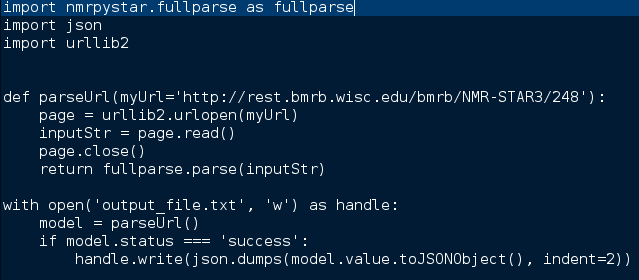
\includegraphics[scale=0.5]{figures/nmrpystar_bmrb}
  \caption[A code snippet of NMRPyStar.]
          {A code snippet of NMRPyStar accessing the BMRB.
           A file is downloaded, then parsed.  Note that in order to use
           the NMRPyStar library, it need only be imported as a regular
           library.  It does not require any external dependencies or
           tedious setup.}
  \label{nmrpystar_bmrb}
\end{figure}

\begin{figure}
  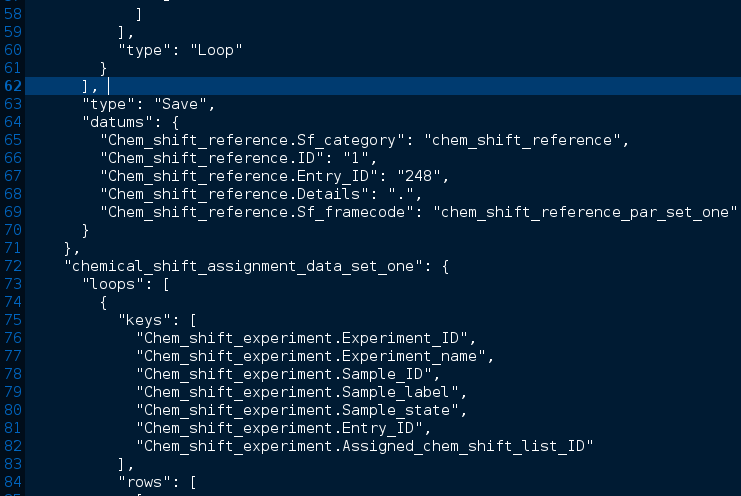
\includegraphics[scale=0.5]{figures/nmrpystar_json}
  \caption[NMRPyStar produces a parse tree as output.]
          {NMRPyStar produces a parse tree as output, shown here in JSON format}
  \label{nmrpystar_json}
\end{figure}

\begin{figure}
  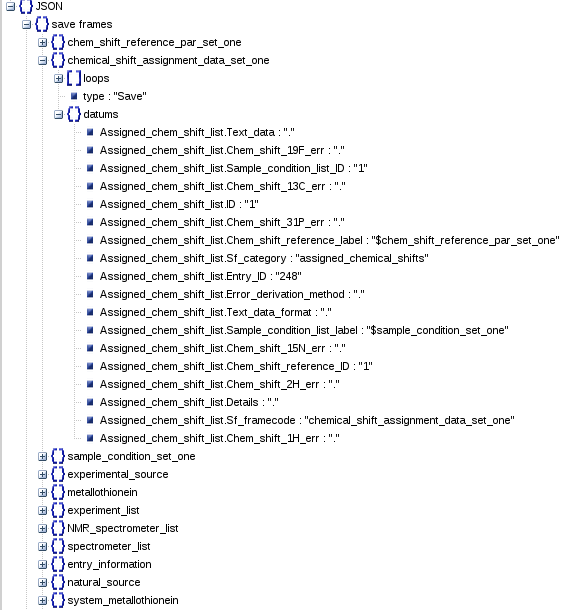
\includegraphics[scale=0.5]{figures/nmrpystar_structure}
  \caption[The parse tree can be used to extract key NMR information.]
          {The parse tree can be used to extract key NMR information.
           It is far easier to query a structured tree than to query
           a flat, unstructured string.}
  \label{nmrpystar_structure}
\end{figure}

\begin{figure}
  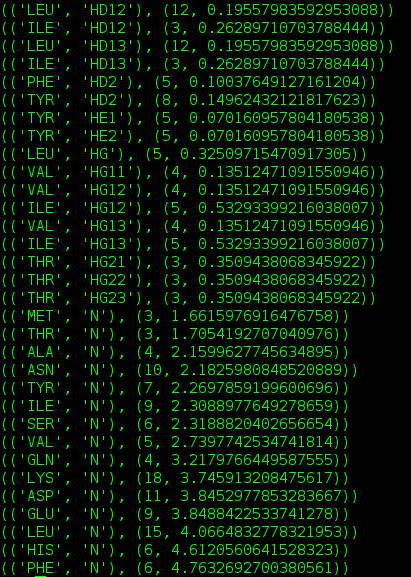
\includegraphics[scale=0.5]{figures/nmrpystar_query}
  \caption[The results of a query run against the parse tree.]
          {The results of a query run against the parse tree.
           The query groups the assigned chemical shifts by
           amino acid type and resonance type, and calculates the 
           standard deviation of each group.  The first column
           is the amino acid name.  The second column is the resonance type.
           The third column is the number of measurements, and
           the fourth column is the standard deviation of the
           measurements.}
  \label{nmrpystar_query}
\end{figure}

\begin{figure}
  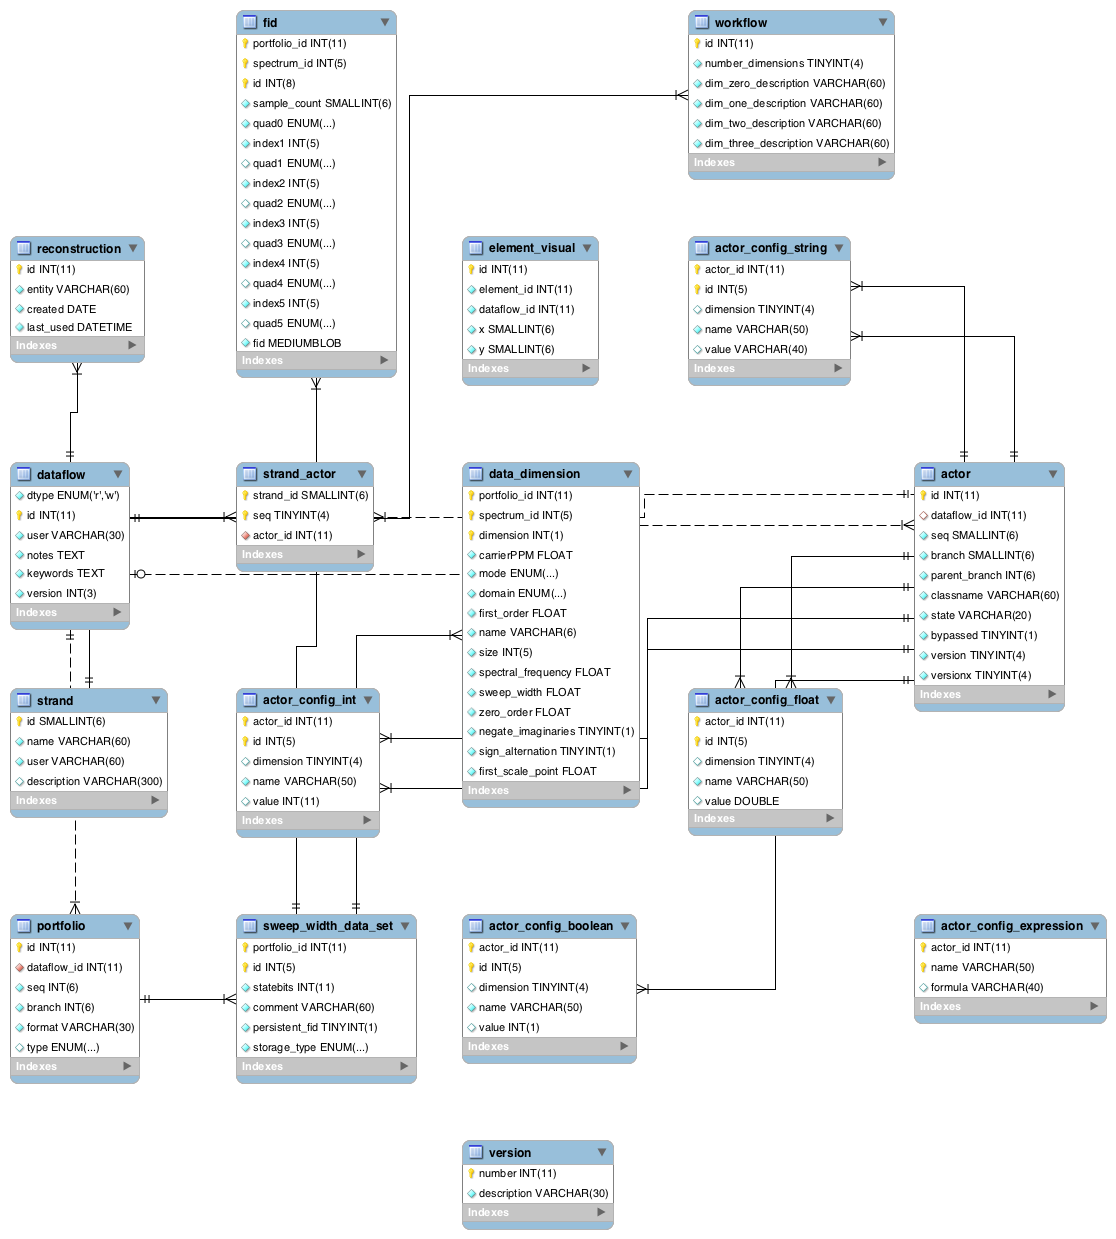
\includegraphics[scale=0.35]{figures/wb_model}
  \caption{WB's data model, created with MySQLWorkbench.}
  \label{wb_model}
\end{figure}

\begin{figure}
  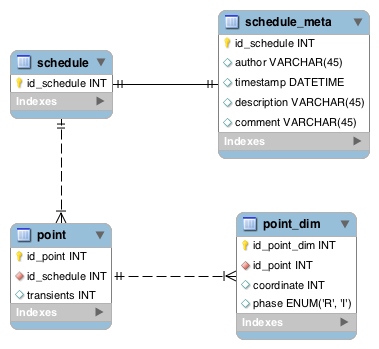
\includegraphics[scale=0.5]{figures/schedule_model}
  \caption{A data model of sample schedules, created with MySQLWorkbench.}
  \label{schedule_model}
\end{figure}

\begin{figure}
  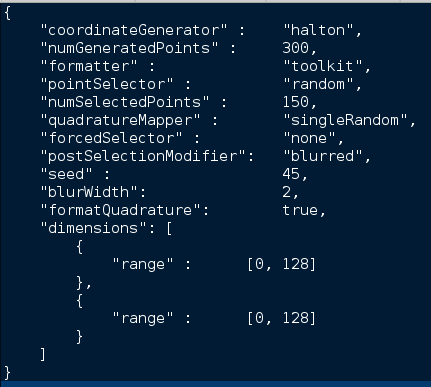
\includegraphics[scale=0.75]{figures/schedule_parameters}
  \caption{The parameter file input for a sample schedule.}
  \label{schedule_parameters}
\end{figure}

\begin{figure}
  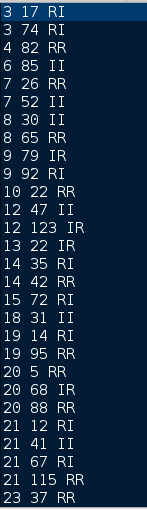
\includegraphics[scale=0.75]{figures/schedule_data}
  \caption{A sample schedule generated from the parameter file.}
  \label{schedule_data}
\end{figure}

\begin{figure}
  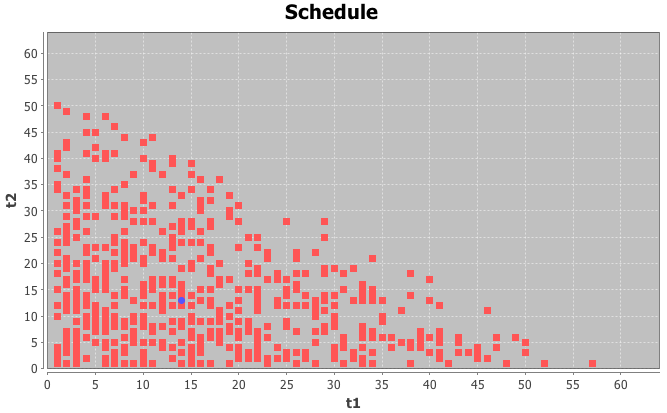
\includegraphics[scale=0.5]{figures/sched1}
  \caption{A graphical view of a sample schedule.}
  \label{sched1}
\end{figure}

\begin{figure}
  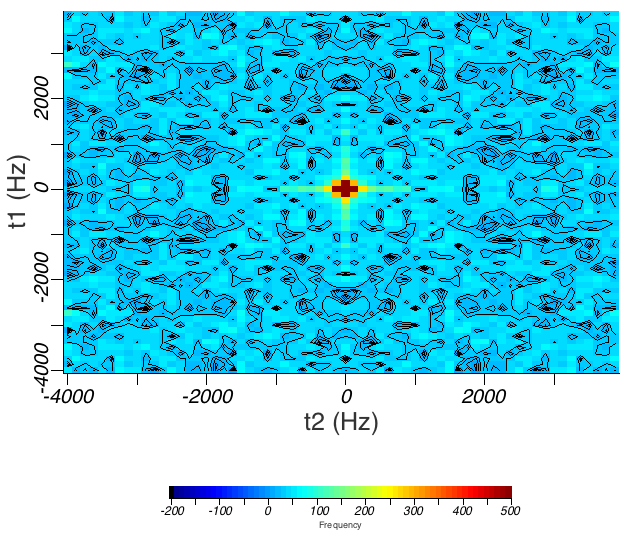
\includegraphics[scale=0.5]{figures/fft1}
  \caption{A sample schedule for which the first points along
           each axis are collected.}
  \label{fft1}
\end{figure}

\begin{figure}
  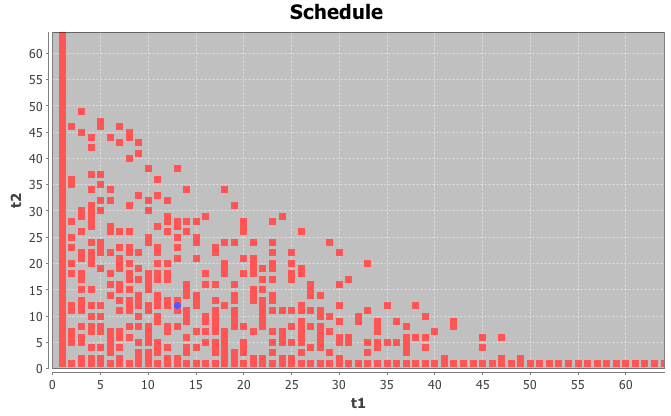
\includegraphics[scale=0.5]{figures/sched2}
  \caption{The pointspread function of the sample schedule, 
           calculated using a real-only FFT.}
  \label{sched2}
\end{figure}

\begin{figure}
  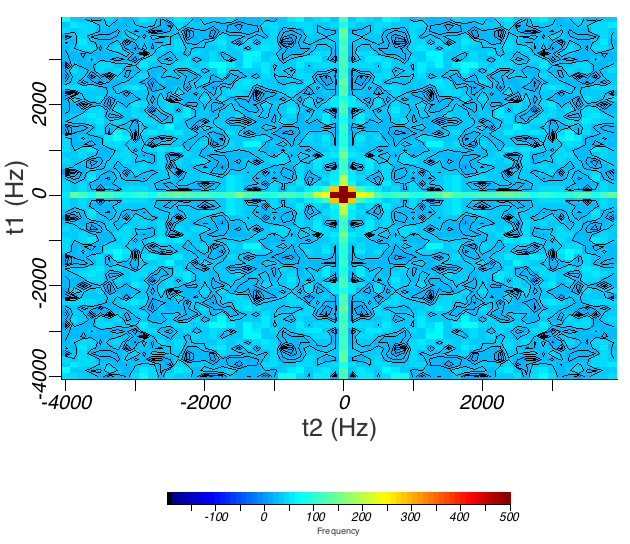
\includegraphics[scale=0.5]{figures/fft2}
  \caption{The pointspread function shows a noticable difference.}
  \label{fft2}
\end{figure}

